\chapter{Calculateur de vol}\label{cha:glide}
Ce chapitre explique comment le calculateur de vol XCSoar fonctionne. Il est recommandé de le lire afin de connaitre les détails spécifiques aux calculs de navigation et de savoir se servir correctement du logiciel. Des connaissances basiques du vol sur la campagne sont présupposées. Les pilotes de compétitions ainsi que les vélivoles occasionnels n'ont rien à perdre à le lire!

\section{Les modes de vol} 
XCSoar accompli différents calculs et affiche différentes InfoBoxes (boîtes d'affichage) en fonction du mode de vol, par exemple "Spirale", "Transition", "Arrivée". XCSoar détecte automatiquement le passage entre le mode "Spirale" et le mode "Transition". 30 secondes en spirale et le calculateur passe du mode "Transition" au mode "Spirale". 30 secondes de vol en ligne droite après la sortie de spirale il passe en mode "Transition".

Le mode "Transition" comporte deux sous-modes : le mode "Arrivée" et le mode "Croisière". Le mode "Arrivée" est activé quand le dernier point de virage est activé ou bien quand le mode "Abandon" est activé lui aussi.

Le passage d'un mode à l'autre est automatique. "Spirale" est activé quand le planeur tourne (environ 3/4 de tour). Il est possible d'activer le mode Spirale par l'intermédiaire d'un matériel externe (un bouton bascule utilisé par le pilote par exemple).

Un petit symbole est affiché en bas à droite de la carte indiquant le mode de vol courant du calculateur.

\begin{tabular}{c c c c}%{c c c c}
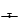
\includegraphics[angle=0,width=0.75cm,keepaspectratio='true']{icons/mode_cruise.pdf} &

\includegraphics[angle=0,width=0.75cm,keepaspectratio='true']{icons/mode_climb.pdf} &

\includegraphics[angle=0,width=0.75cm,keepaspectratio='true']{icons/mode_finalglide.pdf} &

\includegraphics[angle=0,width=0.75cm,keepaspectratio='true']{icons/mode_abort.pdf}\\
(a) & (b) & (c) & (d)
\end{tabular}

\begin{description}
\item[Transition (a)]   Le planeur ne spirale pas et soit il n'y a pas de circuit en cours activé, soit le prochain point de virage n'est pas le dernier.
\item[Spirale (b)]  Le planeur est en spirale (même s'il ne monte pas).
\item[Arrivée (c)]  Le planeur ne spirale pas et le point de virage actif est le dernier du circuit.
\item[Abandon (d)]  Ce mode activé manuellement affiche les différents terrains/zones "posables". (voir section~\ref{sec:taskabort}) 
\end{description}

Les différents calculs que fait XCSoar dépendent bien entendu du mode de vol. L'affichage est différent entre les modes:
\begin{description}
\item Les InfoBoxes  qui peuvent être configurées différemment pour chaque mode de vol.
\item Le zoom spécifique au mode spirale ("zoom spirale").
\end{description}

En plus de ces différents mode d'affichage, un ensemble d'InfoBoxes auxiliaires est disponible. Ces InfoBoxes peuvent-être affichées dans n'importe quel mode de vol. Ceci est utile si le pilote souhaite visualiser des informations dans n'importe quel mode de vol. On y accède par le menu:
\begin{quote}
\bmenu{Info ..}\blink\bmenu{Aux Info On}
\end{quote}

qui permet de basculer entre l'affichage spécifique au mode de vol en cours et l'affichage configuré des InfoBoxes auxiliaires.

Le mode "Arrivée" remplace le mode "Transition" dés que le planeur se trouve au-dessus du plan d'arrivée. L'altitude requise dépend principalement du calage MacCready, mais aussi de la hauteur du relief le long de la route. En prenant un thermique en mode "Arrivée"  XCSoar passe en affichage "Spirale" et en quittant le thermique, repasse en affichage "Arrivée" si les conditions d'arrivée sont remplies (le planeur est au-dessus du plan d'arrivée, toujours en fonction du calage MC et du relief). Pour des circuits courts, il arrive de pouvoir être en arrivée avant de passer l'avant dernier point de virage.

\section{Calage MacCready}

Le calage MacCready peut être fait de plusieurs façons:
\begin{itemize}
\item Depuis le menu
\begin{quote}
\bmenu{Config}\blink\bmenu{MacCready $+$/$-$}
\end{quote}

\item Pour les écrans tactiles/les souris, et utiliser les touches Haut/Bas.
\item Quand un variomètre (supporté) est connecté, le réglage du MC sur le vario change le réglage MC du calculateur XCSoar conformément aux réglages de synchronisation du vario (voir 
  section~\ref{conf:comdevices}).
\end{itemize}
De plus le mode MacCready automatique existe, voir section~\ref{sec:auto-maccready}.

\section{Polaire}
La définition des polaires de nombreux planeurs de différentes classes est intégrée dans XCSoar. Si votre planeur n'est pas dans la liste, le choix d'un planeur aux performances voisines mais pas supérieures peut servir de réglage approximatif. Bien entendu, pour des calculs précis, il faut utiliser la polaire correspondant à votre planeur\config{polar}. Il n'y a pas que la bonne polaire à définir: pour des calculs précis, la masse totale du planeur en vol doit être définie dans XCSoar. XCSoar n'a pas de paramètre "poids du pilote". Pour traduire ce poids vous pouvez utiliser soit la masse totale à vide soit les ballasts.

La polaire est modifiable en vol, afin de tenir compte des moucherons et des vidanges de ballasts.

L'accumulation de moucherons sur le bord d'attaque, la pluie sur les ailes affectent les performances aérodynamiques. C'est au pilote d'évaluer la dégradation des performances aérodynamiques et de modifier la polaire en vol. La valeur de la dégradation estimée est représentée par un pourcentage de dégradation par rapport à la polaire parfaite (100\%). Exemple : à gauche la polaire parfaite, les performances sont à 100\% de la polaire idéale. A droite une dégradation estimée très importante de 50\%. Le taux de chute du planeur est alors le double de celui de la polaire idéale. Les calculs de dégradation sont linéaires. 

\begin{center}
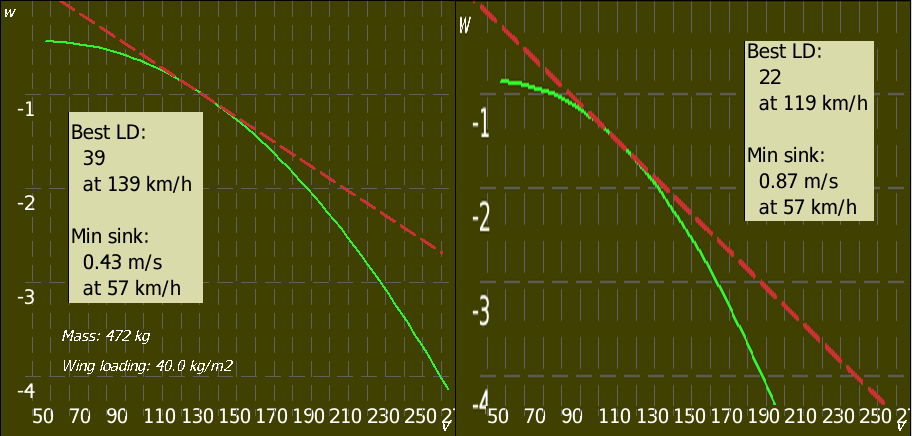
\includegraphics[angle=0,width=\linewidth,keepaspectratio='true']{figures/cut-clean-dirty-polar.png}
\end{center}
Sachant cela, un réglage censé de la valeur de la dégradation de la polaire est important. La valeur correcte est difficile à évaluer. Seuls des tests permettrons de pouvoir connaitre les valeurs correctes, en fonction de la quantité de moucherons et/ou de pluie. Ces valeurs ne ne sont pas identiques d'un planeur à l'autre. 

Le paramètre "Ballast" représente un pourcentage d'eau utilisée par rapport à la capacité totale du planeur. En fonction de la définition de la polaire (menu "config." + "Options Système") il est possible de l'utiliser comme marge suivant le poids des pilotes. A vide, un pilote lourd peut mettre une valeur "Ballast" de 15 litres pour que la polaire soit correctement ajustée à l'accroissement de la masse à vide.

\section{Paramètres de vol}\label{sec:flight-setup}
Ce panel permet de modifier la masse totale du planeur avant et pendant le vol et de régler le QNH. 

On l'affiche par le menu: 
\begin{quote}
\bmenu{Config}\blink\bmenu{Options Vol}
\end{quote}

\begin{center}
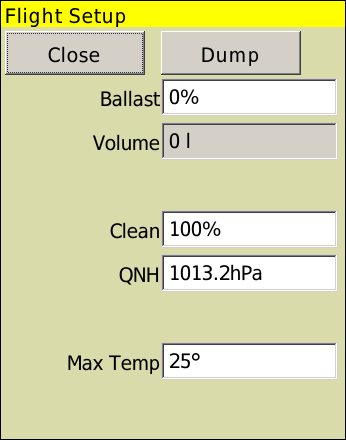
\includegraphics[angle=0,width=0.45\linewidth,keepaspectratio='true']{figures/dialog-basicsettings.png}
\end{center}

Le paramètre "Propreté" défini la performance aérodynamique de l'aile en fonction des moucherons collés sur le bord d'attaque au cours d'un long vol. Si "Propreté" est réglé à 100\% XCSoar utilise la polaire idéale. Un réglage à 50\% dégrade la polaire et double le taux de chute à une vitesse donnée.

Le paramètre "ballast" (en litre) permet de modifier la polaire pour prendre en compte la masse totale du planeur. 

Le réglage du QNH est possible au sol et en l'air. XCSoar utilise cette valeur pour convertir les niveaux de vol en altitudes. Si le logiciel est connecté à un vario supporté muni d'un capteur de pression, l'altitude et le QNH sont mis à jour dans ce panel. Cela permet aussi de caler le QNH au sol en connaissant l'altitude du terrain.

La température maximale prévue au sol est utilisée par l'algorithme de prévision de convection (voir section~\ref{sec:convection-forecast}) pour le calcul de prévision de la hauteur de la base des nuages et du plafond de la convection.

\tip Il est possible de configurer XCSoar pour afficher les paramètres de base au démarrage.

Au démarrage, une fois que le GPS a détecté suffisamment de satellites,  et si un appareil délivrant la pression atmosphérique est connecté  (ex :\ Vega, AltairPro, FLARM), la mise à jour du QNH est automatique. Ce réglage du QNH fait en sorte que l'altitude barométrique corresponde à celle du terrain.

Le QNH est mis à jour uniquement si l'appareil est au sol depuis plus de 10 secondes, afin que si XCSoar est redémarré en vol, le QNH ne soit pas remis à jour. La mise à jour automatique n'est possible que si l'appareil se situe sur un terrain de la base de données.

\section{Affichage vitesse à suivre}

Quand le calculateur est connecté à un instrument délivrant la mesure de la vitesse indiquée, un indicateur de vitesse à suivre est affiché sur la droite de la carte sous la forme de chevrons. Si la vitesse du planeur est inférieure à la vitesse à suivre, des chevrons rouges pointant vers le bas sont affichés. Si le planeur vol trop vite, ce sont des chevrons vers qui pointent vers le haut. Si la vitesse du planeur est optimale, il n'y a pas de chevrons.

En fonction de la configuration, l'affichage de la vitesse à suivre se fait à droite de la carte ou bien dans le cadran du vario.

\section{Vitesse de vol}\label{sec:stf}

XCSoar calcule en permanence 2 vitesses de vol:
\begin{description}
\item[Vitesse MacCready]  La meilleure vitesse en ligne droite et en air calme. Prend en compte le vent en mode "Arrivée".
\item[Vitesse de vol en dauphin]  C'est la meilleure vitesse instantanée en vol en dauphin. Prend en compte le vent en mode "Arrivée".
\end{description}  

Le pilote peut configurer une vitesse de manœuvre maximum qui limite la vitesse calculée MacCready, à des valeurs réalistes.

Les pilotes peuvent avoir leur préférences lors des transitions entre ascendances : le vol MacCready à vitesse constante entre 2 thermiques ou le vol en 'dauphin' qui demande de voler à des vitesses variables.

%\begin{maxipage}
\begin{center}
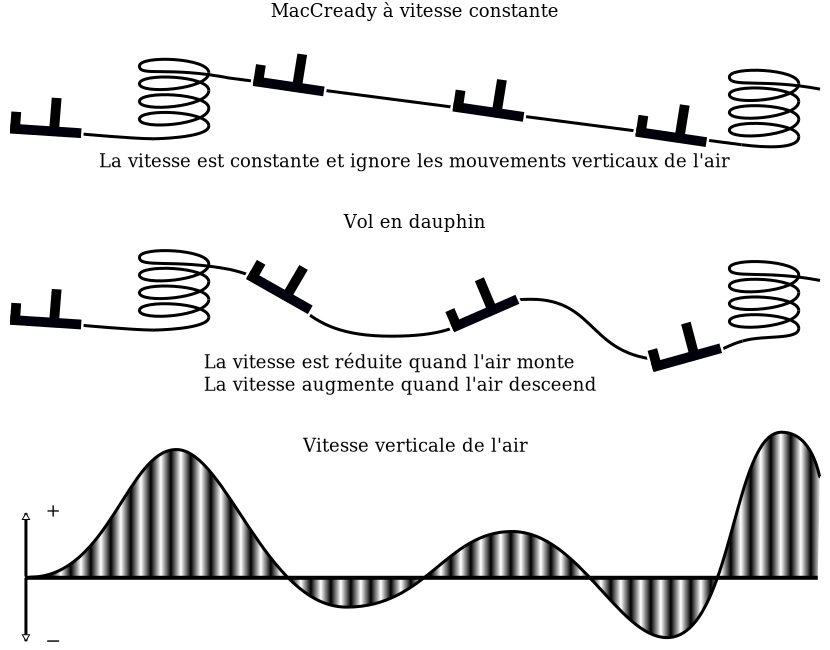
\includegraphics[angle=0,width=1.0\linewidth,keepaspectratio='true']{figures/figure_speed_to_fly-fr.pdf}
\end{center}
%\end{maxipage}

Un paramètre de configuration 'Vitesse de croisière bloquée' (voir section~\ref{sec:final-glide}) peut-être utilisé afin de définir le type de vitesse de vol calculée. L'InfoBoxe 'V Opt' montre la vitesse optimale selon le type de calcul qui est sélectionné. Connecté à un vario Vega, les sons de la "vitesse à suivre"  reflètent cette vitesse.  

\section{Vitesse de vol MC et risque}\label{sec:speed-fly-with}
Le calcul de vitesse de vol peut être compensé en fonction du risque (risque ~= vache  ~= altitude ), dans lequel le calage MacCready utilisé pour les calculs de la vitesse de vol (MC vitesse constante et vitesse en dauphin) est réduit quand le planeur se rapproche du sol.

De nombreux pilotes diminuent le calage du MC quand ils perdent de l'altitude et se rapprochent du sol : cette fonctionnalité le fait automatiquement. Les méthodes de calcul de XCSoar sont basées sur la publication de John  Cochrane, ``MacCready Theory with Uncertain Lift and Limited  Altitude'' {\em Technical Soaring} 23 (3) (Juillet 1999) 88-96.

\url{http://download.xcsoar.org/papers/john.cochrane/safety_glides.pdf}

Un paramètre de configuration $\gamma$ (`Coef. risque sur calage', dans le menu Config ... dans la page 'Paramètres de sécurité')  contrôle comment le "risque MC" est calculé. Le facteur $\gamma$ est une fonction faisant varier le calage MC pris en compte pour les calculs de la vitesse optimale. Il prend en considération la hauteur de la masse d'air convective "utilisable" par le pilote : celle-ci est définie par la hauteur ($h_{top}$) maxi au dessus du sol atteinte en ascendance (généralement proche de la base des nuages). Le paramètre $\gamma$ représente en fait la fraction ($h/h_{top}$) de la hauteur au dessus du sol  ($h$) à laquelle le pilote souhaite abandonner le circuit (se met en prise de terrain pour se vacher ou se dirige vers un point de virage posable) sur la hauteur "utilisable" par le pilote (altitude max des ascendances moins altitude du sol). Une valeur faible de $\gamma$  traduit l'acceptation d'une prise de risque plus importante qu'une valeur importante de  $\gamma$ . 

Si  $\gamma$  est laissé à la valeur par défaut (0.0) il n'y pas pas de compensation (diminution) du calage MC lorsque le sol se rapproche. Pour  $\gamma$  réglé à 1.0, la compensation du MC est linéaire au rapport   $h/h_{top}$. Pour des valeurs intermédiaires de  $\gamma$, la valeur de la compensation MC varie graduellement de façon à compenser de plus en plus en se rapprochant des basses couches.

Des valeurs faibles de  $\gamma$  sont préférables pour les pilotes ne souhaitant pas ralentir quand ils se rapprochent du sol (assument le risque de vache et recherchent la vitesse optimale). Des valeurs élevées de  $\gamma$  doivent être utilisées par les pilotes prudents qui ne recherchent pas la vitesse moyenne maximale.

Une valeur de  $\gamma$  = 0.3 est un bon compromis.

\begin{center}
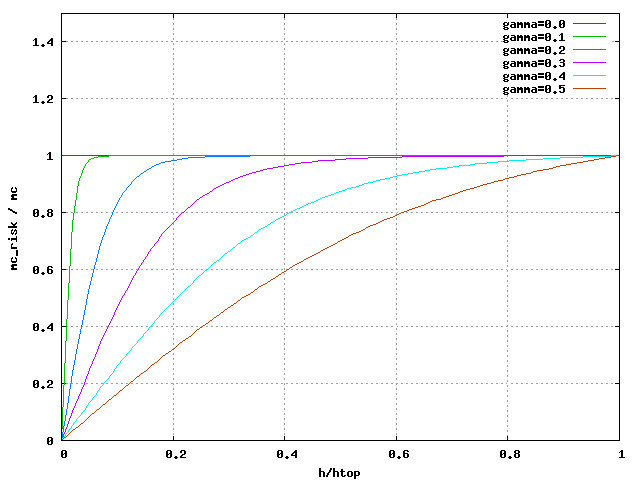
\includegraphics[angle=0,width=0.9\linewidth,keepaspectratio='true']{figures/riskmc.png}
\end{center}

\section{Hauteurs de sécurité}\label{sec:safety-heights}
Trois paramètres de hauteur de sécurité existent dans XCSoar afin de pouvoir définir différentes marges de sécurité, par rapport au sol.
\\
Ces marges sont:
\begin{description}
\item[Hauteur d'arrivée (a)]  Hauteur sol à laquelle le planeur doit arriver pour un atterrissage en sécurité (prise en compte du tour de piste), additionnée d'une marge de sécurité traduisant les  approximations et erreurs des calculs et les incertitudes liées à l'aérologie et au relief. Cette valeur est utilisée dans les calculs d'arrivée ainsi que dans la recherche et l'affichage des terrains atteignables (qui sont en "local").
\item[Garde au sol (b)] Hauteur minimum au-dessus du sol qu'une route calculée doit respecter pour être valide. La garde au sol impacte le calcul de la "zone atteignable en plané". Si le long de la trajectoire prévue d'arrivée la garde au sol n'est pas respectée, une épaisse croix rouge apparait à l'endroit de la violation de la garde au sol. Si la carte des reliefs n'est pas valable ou hors de portée, le calcul de "zone atteignable en plané" et l'affichage de la croix sont désactivés. 
\item[Hauteur de dégagement]  Hauteur sol en dessous de laquelle le pilote décide soit de se vacher, soit d'abandonner le circuit afin de rechercher un terrain posable. Aujourd'hui cette hauteur de dégagement n'impacte en aucune façon les calculs de XCSoar, mais il en est fait référence dans le manuel d'utilisation.
\end{description}

%\begin{maxipage}
\begin{center}
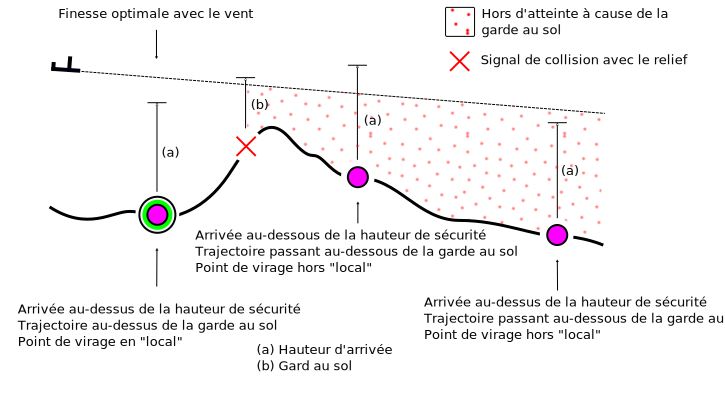
\includegraphics[angle=0,width=\linewidth,keepaspectratio='true']{figures/figure_terrain-fr.pdf}
\end{center}
%\end{maxipage}

\warning
Ces hauteurs de sécurités peuvent être mises à zéro. Mais ceci est tout à fait déconseillé car tout les calculateurs de vol, instruments et sources de données (carte du relief par exemple) sont sujets à erreurs et/ou imprécisions. De plus la masse d'air dans laquelle le planeur évolue est instable et soumise à des évolutions à caractère aléatoire.

XCSoar évalue l'altitude au-dessus du niveau de la mer (ASL) de chaque point de virage ou zone d'atterrissage soit à partir du fichier de points de virage, ou si aucune altitude est définie dans le fichier de points de virage, à partir de la carte relief.

\textbf{L'altitude estimée d'arrivée affichée à côté du point de virage posable est calculée par défaut à partir de la meilleure finesse calculée avec un calage MacCready nul (MC= 0.0) et en tenant compte du vent. Cependant, un calage MC de sécurité, utilisé pour ce calcul,  est paramétrable, comme décrit ci-dessous.}

Les terrains posables sont affichés comme atteignables (en local) si la hauteur estimée d'arrivée par rapport au sol  est supérieure à la hauteur d'arrivée paramétrée et si la trajectoire calculée ne rencontre pas le relief (en tenant compte de la garde au sol).

Dans tout les cas, si le signal de collision apparait (croix rouge), alors le planeur doit reprendre de l'altitude afin d'arriver à destination en sécurité.

Lors du calcul de la hauteur estimée d'arrivée sur les points posables (pour affichage sur la carte et en mode "Abandon"), une valeur de sécurité de calage du MC  est paramétrable dans le menu Config. La valeur par défaut est zéro. Des valeurs plus élevées de ce paramètre rendent le calcul de hauteur d'arrivée plus pessimiste, donc minimisant les risques.

\section{Le calculateur d'arrivée}

Le calculateur d'arrivée utilise de nombreuses sources de données pour déterminer l'altitude nécessaire pour atteindre le point d'arrivée ou le prochain point de virage. Ce sont:

\begin{itemize}
\item La polaire du planeur;
\item La vitesse et la direction du vent;
\item La distance et le cap pour atteindre la cible;
\item Le calage MacCready;
\item L'altitude de la cible;
\item Une hauteur de sécurité spécifique à l'utilisateur (Hauteur d'arrivée).
\item L'énergie totale du planeur si XCSoar est connecté à un instrument lui donnant la vitesse instantanée.
\end{itemize}

Des paramètres ci-dessus découlent deux altitudes:
\begin{description}
\item[Altitude requise] Altitude nécessaire pour atteindre la cible. Cette altitude comprend toute hauteur de sécurité paramétrée.
\item[Hauteur différentielle] calculée à partir de l'altitude nécessaire pour atteindre la cible (incluant la hauteur de sécurité), plus l'altitude de la cible (ASL), moins l'altitude du planeur (ASL). Cette hauteur représente indifféremment la hauteur au-dessus(ou en-dessous) du plan d'arrivée ou bien  la hauteur au-dessus (ou en-dessous) par rapport à la cible. Si aucune altitude n'est définie pour la cible (dans le fichier des points de virage), XCSoar utilise l'altitude de la cible sur la carte du relief.
\end{description}

La méthode de calcul du plan d'arrivée est étendue au calcul des 'altitudes requises' et des 'hauteurs différentielles'  pour terminer le circuit. On parle parfois de cette fonctionnalité comme étant le calcul constant du plan d'arrivée. La hauteur différentielle pour terminer le circuit est affichée en permanence sur la partie gauche de la carte et est représentée sous forme de flèche et de chiffres. 

La hauteur requise est convertie en énergie potentielle, ceci afin de pouvoir prendre en compte l'énergie cinétique du planeur et la convertir en énergie potentielle. L'énergie cinétique qui est convertible en hauteur est calculée à partir de la différence entre la vitesse instantanée et la vitesse à finesse max. Cette valeur sera nettement plus précise si XCSoar est connecté à un instrument lui donnant la vitesse instantanée. Sinon la vitesse "instantanée" est estimée à partir de la vitesse estimée du vent et de la vitesse sol (gps). 

\section{Hauteur différentielle}

Affichage de la hauteur différentielle : sur la partie gauche de la carte, une case affiche la hauteur nécessaire pour terminer le circuit, ou atteindre le point de virage final. Si le planeur est au-dessus de l'altitude minimum requise, au-dessus de la case, une flèche verte pointe vers le haut. Si le planeur est en-dessous du minimum requis une flèche rouge pointe vers le bas, représentant le manque de hauteur pour atteindre la cible. Si cependant il y a des zones posables en "local" mais que le planeur est en déficit de hauteur pour terminer le circuit, la flèche est de couleur ambre.

\begin{center}
\begin{tabular}{c c}
{\it Au-dessus} & {\it Au-dessus} \\
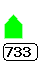
\includegraphics[angle=0,width=0.15\linewidth,keepaspectratio='true']{figures/cut-fg-above.png} &
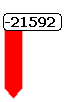
\includegraphics[angle=0,width=0.2\linewidth,keepaspectratio='true']{figures/cut-fg-below.png} \\
\end{tabular}
\end{center}

L'échelle de la flèche d'arrivée est $+/-$ 500 mètres.

\subsection*{Double flèche et hauteur différentielle}

La flèche d'arrivée a été modifiée pour montrer l'effet du calage MC sur la hauteur différentielle nécessaire pour terminer le circuit. L'affichage d'une flèche creuse montre la hauteur différentielle avec un calage MC à zéro, tandis que la flèche pleine affiche la hauteur différentielle avec le calage MC actuel.

Le nombre dans la boite à la base de la flèche montre toujours la hauteur différentielle calculée avec le calage MC actuel.

Exemples d'affichages dans différentes situations:

\begin{description}

\item[Au-dessus du plan à MC$=M$ et MC$=0$]
  Ici la flèche verte pleine montre la hauteur haut-dessus du plan d'arrivée calculée avec le calage MC courant(M). La flèche creuse représente la hauteur additionnelle en excès.

\begin{center}
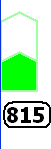
\includegraphics[angle=0,width=1.6cm,keepaspectratio='true']{figures/fig-finalglide-allabove.png}
\end{center}

\item[Au-dessous du plan à MC$=M$, et au-dessus à MC$=0$]
  Ici on voit qu'avec le calage MC courant le planeur est au-dessous du plan (flèche rouge). La flèche verte creuse montre qu'avec un calage MC$=0$, le planeur est au-dessus du plan d'arrivée.  

Dans cette situation, si le planeur monte, le pilote doit alors prendre une décision: soit quitter le thermique tôt et commencer sont arrivée avec un calage MC faible, soit continuer à spiraler. Il est utile de passer en MC auto afin d'avoir comme directive la valeur optimale de calage MC  --- alors il est facile au pilote de comparer son ascendance moyenne réalisée avec le calage MC optimal calculé. Quand la Vz moyenne est inférieure au calage MC proposé, il est temps de quitter le thermique.

\begin{center}
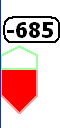
\includegraphics[angle=0,width=1.6cm,keepaspectratio='true']{figures/fig-finalglide-halfabove.png}
\end{center}

\item[Sous le plan à MC$=M$, et à peine sous le plan à MC$=0$]
  Ici on voit qu'au calage MC courant, le planeur est bien au-dessous du plan (flèche rouge). La flèche creuse rouge montre qu'en réduisant le calage MC à zéro, le planeur est presque dans le plan d'arrivée.
\begin{center}
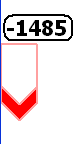
\includegraphics[angle=0,width=2cm,keepaspectratio='true']{figures/fig-finalglide-littlebelow.png}
\end{center}

\item[Sous le plan à MC$=M$, ainsi qu'à  MC$=0$]
  Ici on voit qu'au calage MC courant, le planeur est bien au-dessous du plan (flèche rouge). Il n'apparait pas de flèche creuse. Ceci signifie que même à un calage MC$=0$, le planeur est bien en-dessous du plan d'arrivée.
\begin{center}
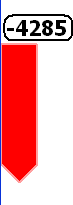
\includegraphics[angle=0,width=2cm,keepaspectratio='true']{figures/fig-finalglide-allbelow.png}
\end{center}
\end{description}
 

\section{Estimation de la vitesse sur circuit}\label{sec:task-speed-estim}

Certains algorithmes de calcul utilisés par XCSoar se servent de l'estimation des temps requis pour passer chaque point de virage. Cette information est utilisée dans l'affichage de certaines {\InfoBox}, calculs d'AAT et avertissements de coucher de soleil. 

Pour évaluer la vitesse moyenne sur le circuit, le calculateur de vol se base sur la vitesse calculée avec la théorie MacCready classique en prenant en compte la force du vent et sa direction et en utilisant le calage MC courant. cette méthode est utilisée pour calculer les temps d'arrivée aux points de virage et pour l'heure d'arrivée du circuit.

Définition des mesures de différentes vitesses du circuit:
\begin{description}
\item[Vitesse réalisée sur circuit]  Vitesse réalisée jusqu'à présent, tenant compte de la différence entre l'altitude actuelle et celle du départ.
\item[Vitesse moyenne estimée]  Vitesse moyenne du circuit, prenant en compte l'altitude nécessaire pour achever le circuit.
\item[Vitesse restante]  Vitesse estimée pour la partie restante du circuit, basée sur la théorie MacCready.
\item[Vitesse estimée instantanée]  Vitesse estimée instantanée au long du circuit. En montée a une vitesse égale au calage MC, ce chiffre sera équivalent à la vitesse estimée du circuit. En montée lente par rapport au calage MC ce chiffre sera inférieur à la vitesse estimée du circuit. En transition, à vitesse optimum et ascendance nulle, ce chiffre sera égal  à la vitesse estimée du circuit.

Cette vitesse estimée, affichable dans une {\InfoBox}, est utile comme indicateur de performance sur le circuit. Étant une estimation, cette vitesse n'est jamais utilisée dans les calculs internes de XCSoar.
\end{description}

Pour les AAT, quand l'estimation d'heure d'arrivé est calculée, les points de virages sont optimisés. \tip Pour chaque point de virage variable (dans les zones définies du circuit) paramétré à "auto", XCSoar déplace la position du point de virage pour faire en sorte que le circuit soit terminé au plus 5 minutes après le temps imparti de l'épreuve.

La vitesse appelée  {\em MacCready réalisé} est calculée en trouvant le calage MC qui en configuration de vol MC classique produirait la même vitesse sur circuit que la vitesse réalisée. Cette valeur est supérieure au calage MC courant quand le planeur est monté plus rapidement que le calage MC ou lors de vol sous des rues de nuages, etc... Ce {\em MacCready réalisé} est affiché dans le menu \bmenu{NAV.}\blink\bmenu{Circuit} onglet "Calculateur".

L'estimation de la "Vitesse restante" prend en considération les variations d'altitude, comme les effets des montées sont prises en compte pour la "Vitesse moyenne estimée". Considérons 2 planeurs A et B de même type parcourant le même circuit : le planeur A a transité rapidement, privilégiant la vitesse à l'altitude. Le planeur B se retrouve derrière A mais plus haut et gagnera du temps plus tard en ayant moins de hauteur à gagner pour achever le circuit.

Lors de circuit AAT, la "Vitesse restante" varie, quand le planeur est à l'intérieur d'une zone de point de virage AAT, quand la distance du circuit ou le point de virage sont modifiés par le pilote. Ceci est du à la variation de distance restante à parcourir.


\section{Optimisation de la route}
Dans le but de réduire les écarts de route entre deux points de virages (hors point d'arrivée), XCSoar calcule la meilleure route à suivre, la "route optimale". Cette optimisation prend en compte l'écart de route résultant du vol en thermique. Pour cela, il y a estimation du temps nécessaire passé en spirale en accord avec la théorie MacCready classique.

\begin{center}
\begin{maxipage}
\centering
\def\svgwidth{0.8\linewidth}
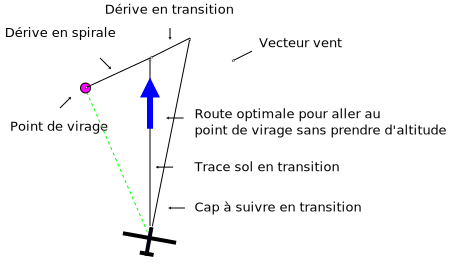
\includegraphics[angle=0,width=0.8\linewidth,keepaspectratio='true']{figures/figure_optimal_cruise-fr.pdf}
\end{maxipage}
\end{center}

La direction de la route optimale est affichée sous la forme d'une flèche bleue épaisse. Elle indique la direction optimale que doit suivre la trace au sol du planeur en transition. Par exemple, si l'affichage est paramétré "Route en haut" il faut se diriger pour faire en sorte que la flèche soit dirigée vers le haut, et donc parallèle à la route.

Le calculateur de vol prend en compte la dérive due au vent lors des spirales afin de donner la direction optimale à suivre : elle indique la route que le planeur devrait suivre en transition afin d'arriver le plus tôt possible au point de virage suivant. Quand le vent est négligeable ou quand le calculateur est en mode "arrivée", la flèche bleue est parallèle à la ligne noire qui indique la direction au prochain point.

Le calcul et l'affichage de la route optimale à suivre est une fonctionnalité que seul XCSoar fourni pour le moment. Généralement, en transition entre les thermiques les systèmes d'aide à la navigation indiquent la route à suivre comme étant simplement la ligne droite menant au prochain point de virage. Le planeur doit idéalement suivre, sur la carte, la droite tracée entre deux points de virage afin de faire le minimum de kilomètres possible. Quand la composante du vent perpendiculaire à cette droite est importante, XCSoar permet facilement de la suivre ou de s'en approcher. 

Toutefois, comme en général le planeur doit prendre des ascendances pour gagner de l'altitude, en spiralant la dérive due au vent peut devenir importante et augmente l'écart à la route directe. Après plusieurs arrêts dans des thermiques, la trace au sol peut devenir une courbe très écartée de la route idéale.

\section{MacCready Auto}\label{sec:auto-maccready}

Pour aider le pilote, XCSoar peut ajuster le calage MacCready automatiquement. Deux méthodes de calage automatique sont possibles:
\begin{description}
\item[En arrivée]  En arrivée, le MC est calé de façon à atteindre le point d'arrivée en un minimum de temps. Pour les épreuves AAT, le calage MC permet de parcourir la distance maximale dans le temps restant de l'épreuve et d'atteindre le point d'arrivée (hauteur d'arrivée prise en compte).
\item[Moyenne des ascendances] En dehors des arrivées, le calage MC est égal à la moyenne de tout les thermiques depuis le début du vol.
\end{description}
Il est possible d'utiliser les deux méthodes : avant de passer en mode arrivée, le calage MC est égal à la moyenne des ascendances rencontrées et lors du passage en arrivée le calage MC s'ajuste de façon à minimiser le temps d'arrivée.

La méthode utilisée se configure dans le menu 'Config' + 'Calculateur de Vol' + 'Calculateur de Vol', avec le champ "Auto MC mode". La valeur par défaut est "Les 2".

Pour activer/désactiver le mode MacCready Auto: 
\begin{quote}
\bmenu{Config}\blink\bmenu{MacCready Auto}
\end{quote}

Quand le MC Auto est activé, l'infobox MacCready affiche 'AUTO' à la place de 'MANUEL'; le MacCready du vario affiche 'MC Auto' au lieu de 'MC'.

Le fonctionnement du MacCready Auto est décrit en détails ci-dessous.

\subsection*{En Arrivée}
Quand le planeur est au dessus du plan d'arrivée, le calage MC peut-être augmenté, ce qui résulte en une vitesse recommandée plus importante. Le fait d'augmenter le calage MC augmente aussi la Vz minimale des thermiques dans lesquels il en rentable de s'arrêter.

De même, quand le planeur est sous le plan d'arrivée, le calage MC peut-être réduit se qui conduit à une vitesse recommandée plus faible. Du fait de la réduction le calage MC, le pilote doit prendre des thermiques plus faibles.

Le MacCready Auto permet de faire varier le calage MC automatiquement et en permanence. En général, il n'a aucun sens à s'en servir avant d'atteindre le plan d'arrivée ou presque. Si activé très/trop tôt, le planeur est alors très en dessous du plan d'arrivée et la fonctionnalité du MacCready Auto conduit à un calage égal à zéro.

\begin{maxipage}
\begin{center}
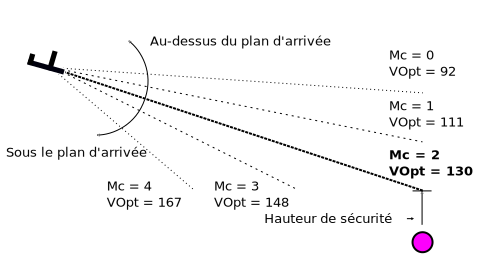
\includegraphics[angle=0,width=0.8\linewidth,keepaspectratio='true']{figures/figure_auto_maccready-fr.pdf}
\end{center}
\end{maxipage}

\subsection*{Moyenne des ascendances}

Cette méthode cale le MC à la valeur moyenne de toutes les ascendances rencontrées au cours du vol. À ce titre, elle prend en compte le temps passé à centrer les thermiques. La valeur est mise à jour à la sortie des thermiques.

Étant donné que la théorie MacCready est optimale si le calage MacCready est égal au taux de montée moyen de la prochaine ascendance, cette méthode peut donner des performances sous-optimales (vitesse recommandée trop lente) si les conditions s'améliorent; et de même elle peut être non conservatrice si les conditions se détériorent (vitesse recommandée trop élevée).  De même, si le pilote continue à monter en thermiques faibles, cela réduira la moyenne et peut donc encourager le pilote à continuer à sélectionner les thermiques faibles.

En raison de ces limitations, le pilote doit être au courant du mode de fonctionnement du système et adapter ses décisions en conséquence.

\section{boîte de dialogue analyse}

La boîte de dialogue analyse peut servir à vérifier la polaire.  Ceci est accessible via le menu
\begin{quote}
\bmenu{Info.}\blink\bmenu{Analyses}
\end{quote}

La page polaire montre le graphique de la polaire avec prise en compte des moucherons et de la charge alaire. Sont aussi affichées les vitesses de finesse max calculée, de chute mini, la masse et la charge alaire.

\begin{center}
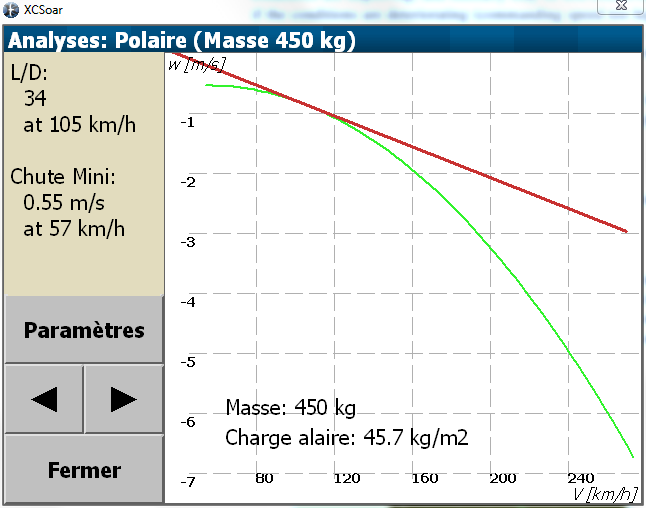
\includegraphics[angle=0,width=0.8\linewidth,keepaspectratio='true']{figures/analysis-glidepolar.png}
\end{center}

Dans cette page de dialogue, le bouton "Paramètres" ouvre la page "Configuration vol" et permet de régler en vol les paramètres 'Moucherons' 'QNH' et 'Temp. max.'.

Quand le calculateur est connecté à un vario "intelligent" et supporté par XCSoar (ex : Vega) la page polaire montre la moyenne de l'énergie totale de descente en vol en fonction de la vitesse horizontale. Cette fonctionnalité permet de réaliser des vols de test en air stable et vent nul afin de mesurer la polaire réelle. En comparant la polaire constructeur à celle mesurée, il est possible de contrôler / optimiser la vitesse de changement de position des volets, l'influence de l'étanchéité des ailerons et volets....  

Les données sont collectées uniquement en vol de transition et à un facteur de charge compris entre 09 et 1,1 G. Les pilotes faisant des vols d'essais doivent donc voler dans un air stable et manœuvrer doucement les commandes. 
\begin{center}
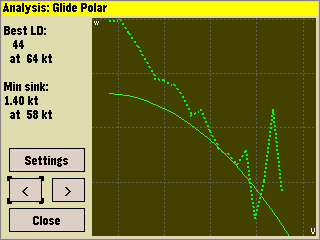
\includegraphics[angle=0,width=0.8\linewidth,keepaspectratio='true']{figures/shot-glidepolar.png}
\end{center}

\section{Notifications de vol}

Les notifications, affichées comme des messages d'état, apparaissent dans les conditions suivantes:
\begin{itemize}
\item Arrivée prévue en avance par rapport au temps donné d'un AAT.
\item Arrivée estimée après le coucher du soleil.
\item Changement important du vent (intensité ou direction).
\item Passage au-dessus ou au-dessous du plan d'arrivée.
\end{itemize}
% JMW more detail here
